% Created 2016-05-01 Son 22:42
\documentclass[11pt, a4paper]{article}
\usepackage[utf8]{inputenc}
\usepackage[T1]{fontenc}
\usepackage{fixltx2e}
\usepackage{graphicx}
\usepackage{longtable}
\usepackage{float}
\usepackage{wrapfig}
\usepackage{soul}
\usepackage{textcomp}
\usepackage{marvosym}
\usepackage{wasysym}
\usepackage{latexsym}
\usepackage{amssymb}
\usepackage{hyperref}
\tolerance=1000
\usepackage{minted}
\usepackage[utf8]{inputenc}
\usepackage[english]{babel}
\usepackage{graphicx}
\usepackage[left=2.35cm, right=3.35cm, top=3.35cm, bottom=3.0cm]{geometry}
\usepackage{titling}
\providecommand{\alert}[1]{\textbf{#1}}

\title{Statistical methods for bioinformatics \linebreak Gene expression: case study (de Vijver et al.)}
\author{Cedric Lood}
\date{\today}
\hypersetup{
  pdfkeywords={},
  pdfsubject={},
  pdfcreator={Emacs Org-mode version 7.9.3f}}

\begin{document}

\maketitle


\graphicspath{ {figures/} }
\setlength{\droptitle}{-5em} 
\setlength{\parindent}{0cm}

\section{Dataset}
\label{sec-1}

The dataset under consideration consists of values of about 5000 gene
expressions (obtained through a microarray technology) for 188
patients. Some of the patients developed distant metastases while
others did not, and the goal is to see if we can use the information
from the levels of gene expressions to predict the metatstases
phenotype and subsequently use appropriate treatment for the patient.

One thing to note from the dimensions of the dataset is that we are
falling in the case of so-called high dimensionality with a number of
observations $n$ that is over an order of magnitude lower than that of
the $p$ predictors. Among other things, this prevents the use of least
square methods, common in linear models. 

One of the risk when trying to come up with a reduced gene panel that
would predict the evolution of the cancer is that high levels of
colinearity between the predictors likely exists. This renders the set
of gene selected contingent on the particular dataset obtained.
\section{Predictive potential}
\label{sec-2}

Here are the libraries I used throughout the analysis:

\begin{minted}[]{R}
library(glmnet)
library(polycor)
library(ROCR)
library(leaps)
library(pls)

load("VIJVER.Rdata")
\end{minted}

As a first approach, I tried to search systematically through the
dataset for variables that would correlate with the binary outcome
with a correlation score above 0.45 (for a score of 0.5, the procedure
returns only 2 results).


\begin{minted}[]{R}
## Systematic identification of correlated genex/outcome
genes <- character()
i <- 1
for(gene in names(data)[2:length(data)]) {
    if(abs(hetcor(data$meta, data[gene])$correlations[1,2]) > 0.45){
        genes[i] <- gene
        i <- i + 1
    }
}
\end{minted}

Here is the list of genes returned:


\begin{verbatim}
 [1] "NM_000987"      "NM_003258"      "NM_003295"      "NM_004119"     
 [5] "NM_004203"      "NM_002808"      "NM_002811"      "NM_012291"     
 [9] "NM_013277"      "NM_003981"      "NM_004701"      "M96577"        
[13] "NM_007019"      "NM_007057"      "NM_007267"      "NM_007274"     
[17] "NM_006607"      "NM_016185"      "Contig48913_RC" "NM_018410"     
[21] "NM_001168"      "NM_002106"
\end{verbatim}

Which I then used to build a logistic model, with a best subset
selection approach. For the selection, I used the BIC metric to
select the subset of variable and obtained a ROC curve for the
classifier obtained (see graphics below).


\begin{minted}[]{R}
## Use the identified variables to create a model
regfit.full <- regsubsets(data.meta~., reduced.data, nvmax = length(genes))
reg.summary <- summary(regfit.full)

## using bic to make a decision, n=4
which.min(reg.summary$bic)
coef(regfit.full,4)

## fitting model with the 4 params
reg <- glm(meta~NM_000987+NM_003258+NM_004119+NM_002811, data=data,family = binomial(link=logit))
summary(reg)
reg.probs <- predict(reg, type="response")
contrasts(data$meta)
table(data$meta, fitted(reg)>0.5)
predict <- fitted(reg)
pred <- prediction(predict, data$meta)
perf <- performance(pred, measure="tpr", x.measure = "fpr")
performance(pred, measure="auc")

## plotting the results
pdf("bic-auc.pdf", width = 16, height = 8)
par(mfrow = c(1,2))
plot(reg.summary$bic, ylab="bic", type="l")
plot(perf, col="red")
dev.off()
\end{minted}

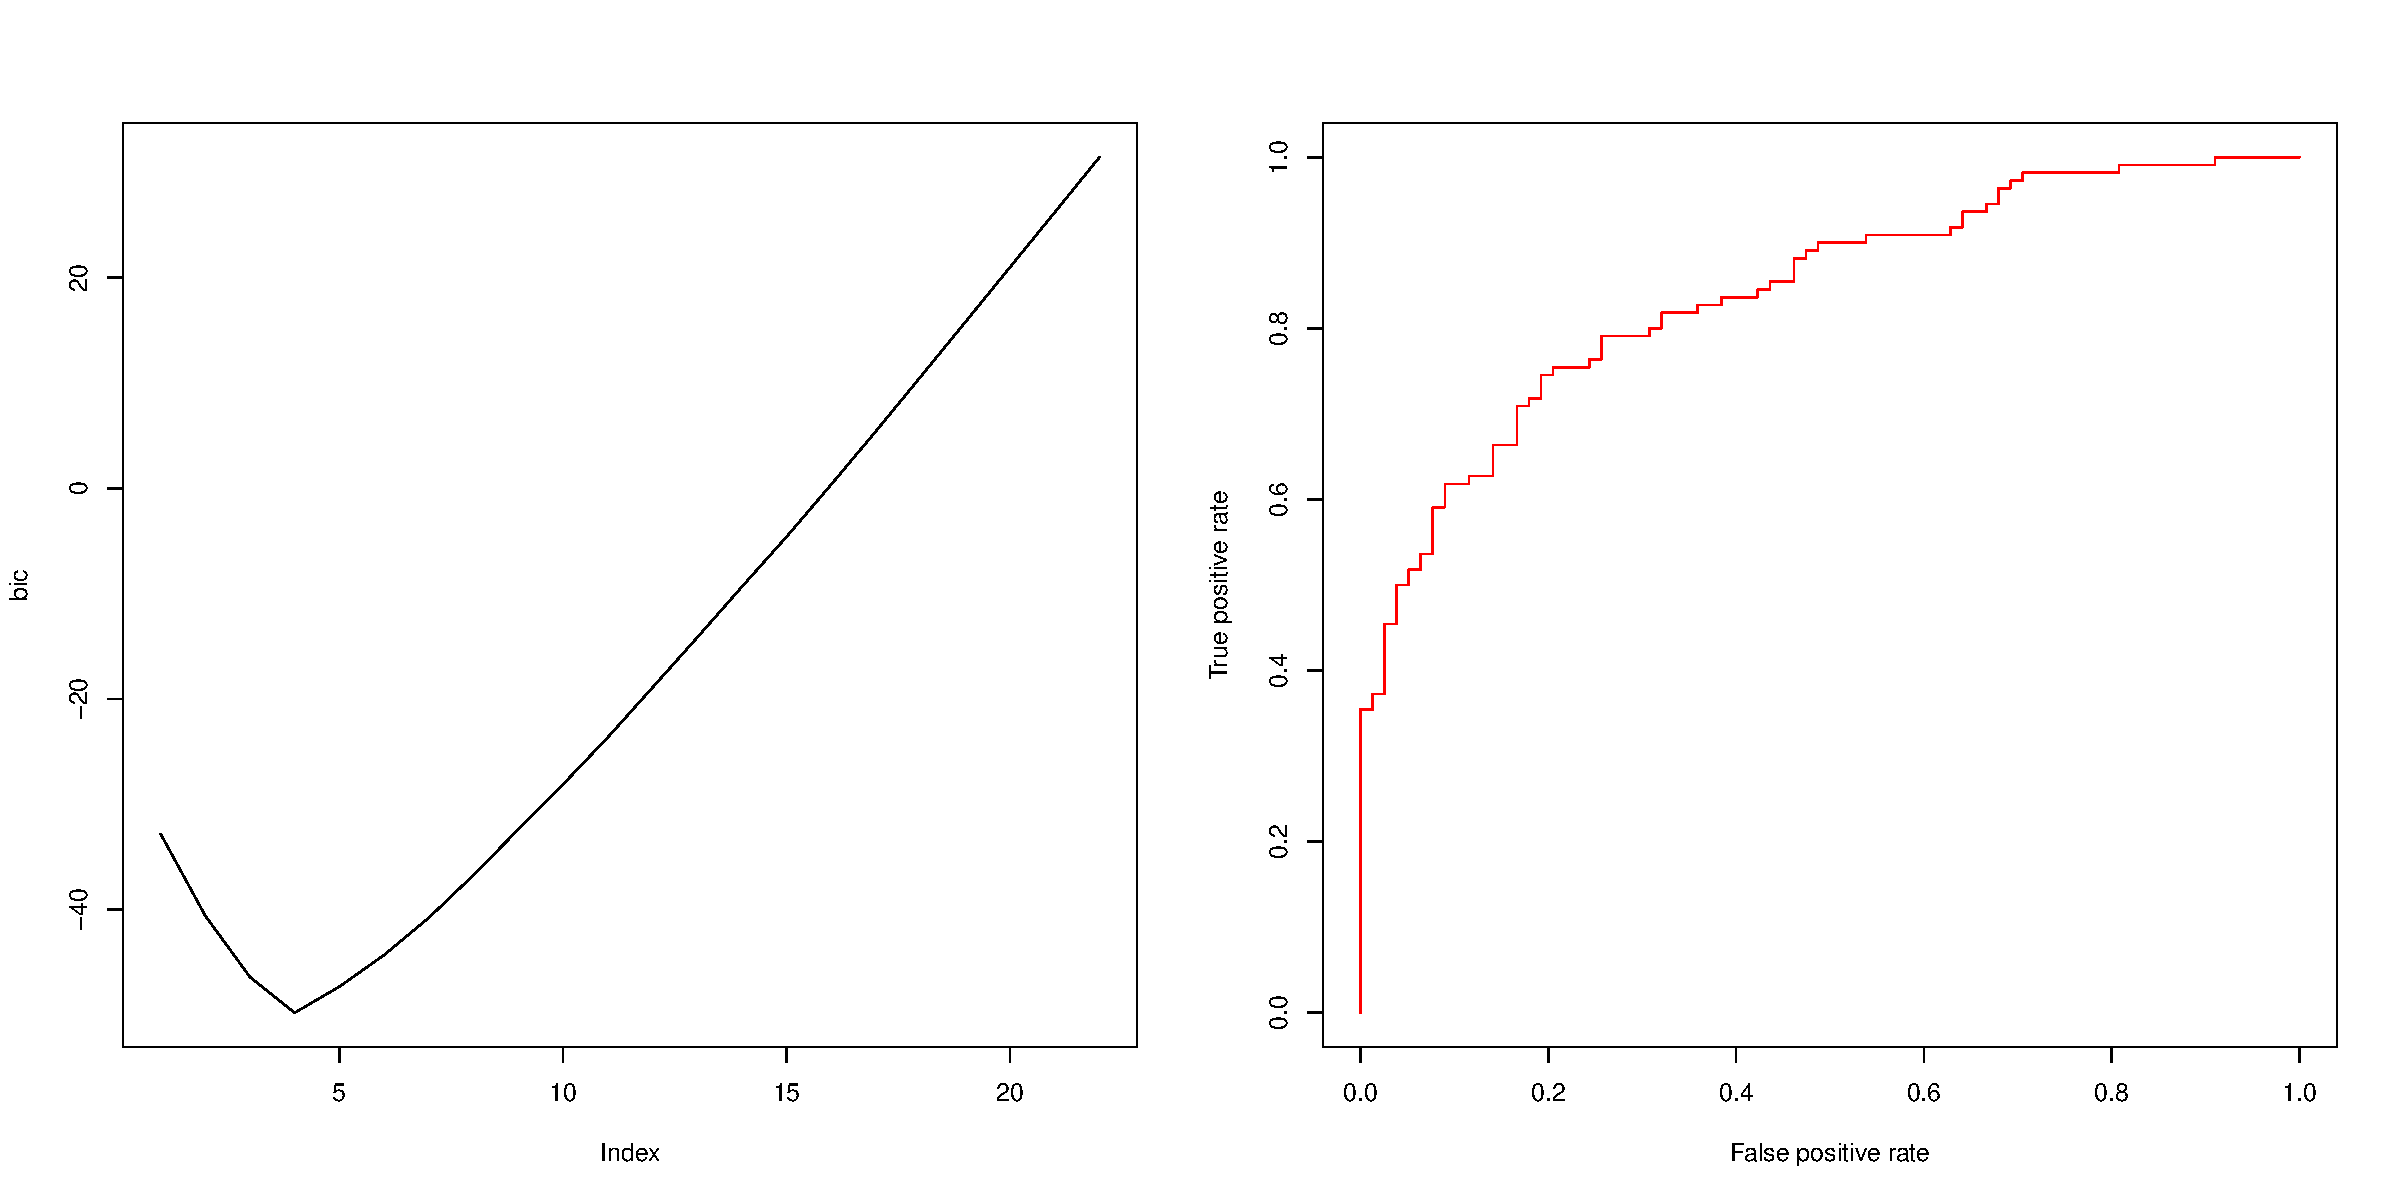
\includegraphics[scale=0.4]{bic-auc.pdf}
\section{Collinearity structure}
\label{sec-3}

Given the size and the nature of the data collected (RNA transcript
levels), we can certainly expect colinearity between different
predictors. One simple justification for it is that often multiple
genes encode the information necessary for a given pathway. Those will
then be transcribed together in order to enable the different steps in
the metabolic pathway to be succesful. 

This represents a challenge in the statistical analysis as colinearity
leads to unstability in the modelling. Typically, the fitted
coefficients of the model will vary significantly with small
perturbations in the dataset.

Working with the reduced dataset of 22 transcript levels created
above, one can alreay show multiple examples of such colinearity:


\begin{minted}[]{R}
pairs(reduced.data[,2:8]) # no good examples in this subset (max=0.5)
cor(reduced.data$NM_002808,reduced.data$NM_002811)
pairs(reduced.data[,9:16]) # good amount of corelated pairs (max=0.9)
cor(reduced.data$NM_003981,reduced.data$NM_004701)
\end{minted}


\begin{verbatim}
> cor(reduced.data$NM_002808,reduced.data$NM_002811)
[1] 0.5072933
> cor(reduced.data$NM_003981,reduced.data$NM_004701)
[1] 0.8694202
\end{verbatim}

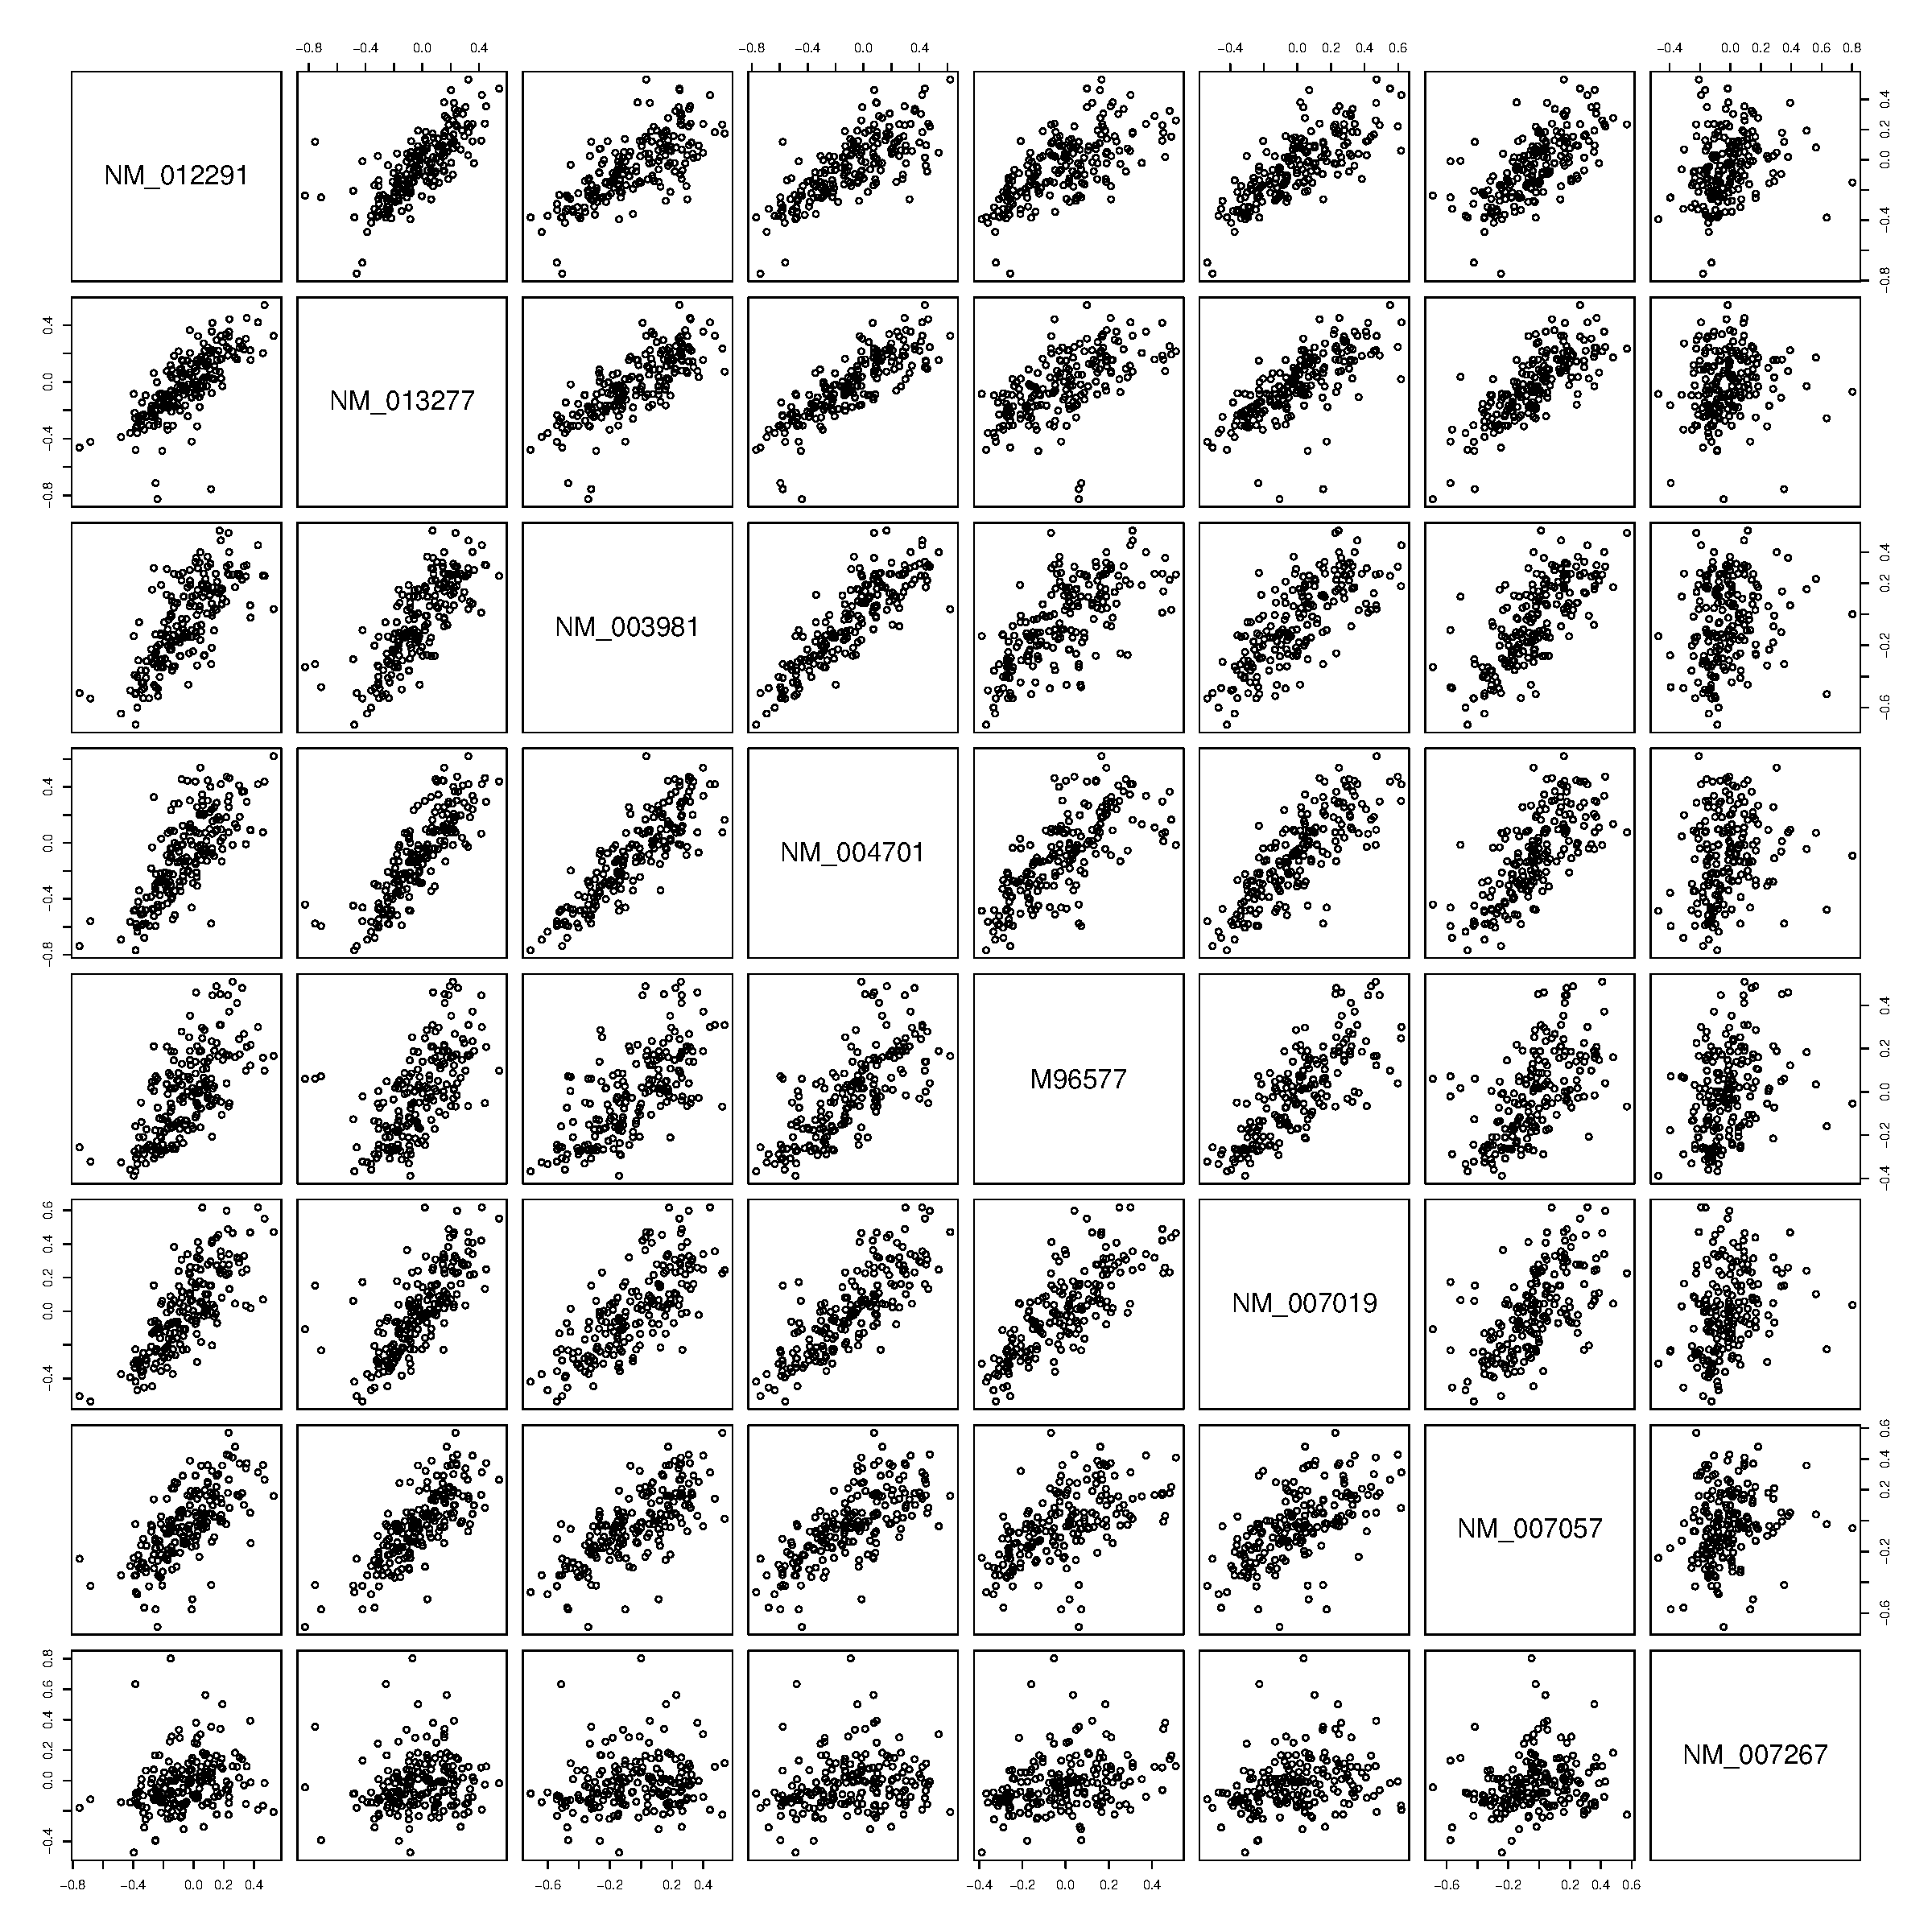
\includegraphics[scale=0.4]{pairs-colinearity.pdf}
\section{Phenotype prediction}
\label{sec-4}


I used the ridge regression and lasso approaches to build
classifiers. Another one was suggested - principal component
regression - but it did not work due to the binary nature of the
response variable. For both approaches, I used CV to determine the
value of the hyperparameter $\lambda$

The ridge regression does not perform variable selection, so all the
coefficients were present, but for lasso, only 30 predictors were kept
in the final model.

Below the source code are some metrics used to measure the quality of
the models and graphs of the ROC for the classifiers.


\begin{minted}[]{R}
set.seed(1)
x <- model.matrix(meta~.,data)[,-1]
y <- data$meta

## Ridge regression with CV
grid <- 10^seq(10,-2,length=100)
ridge.cv <- cv.glmnet(x,y,alpha=0, family='binomial')
plot(ridge.cv)
ridge.bestlam <- cv.out$lambda.min

ridge.mod <-  glmnet(x,y,alpha=0,lambda=grid,family='binomial')
ridge.pred <- predict(ridge.mod, type="response",s=ridge.bestlam, newx=x)
table(y, ridge.pred>0.5)

ridge.pred <- prediction(ridge.pred, y)
ridge.perf <- performance(ridge.pred, measure="tpr", x.measure = "fpr")
performance(ridge.pred, measure="auc")

## Lasso
lasso.cv <- cv.glmnet(x,y,alpha=1,lambda=grid,family='binomial')
plot(lasso.mod)
lasso.bestlam <- lasso.cv$lambda.min

lasso.mod <- glmnet(x,y,alpha=1,lambda=grid,family='binomial')
lasso.coef <- predict(lasso.mod, type="coefficients",s=lasso.bestlam)
lasso.coef[lasso.coef!=0]
lasso.pred <- predict(lasso.mod, type="response",s=lasso.bestlam, newx=x)
table(y, lasso.pred>0.5)

lasso.pred <- prediction(lasso.pred, y)
lasso.perf <- performance(lasso.pred, measure="tpr", x.measure = "fpr")
performance(lasso.pred, measure="auc")

## plotting results of ridge and lasso (ROC)
pdf("roc-lasso-ridge.pdf", width = 16, height = 8)
par(mfrow = c(1,2))
plot(ridge.perf, col="red", main="ridge regression")
plot(lasso.perf, col="red", main="lasso")
dev.off()
\end{minted}


\begin{verbatim}
> lasso.coef[lasso.coef!=0]
<sparse>[ <logic> ] : .M.sub.i.logical() maybe inefficient
 [1]  0.247743870  0.011295692  0.346844990 -0.895657534  0.552269072
 [6] -0.423686469  0.786917703 -1.272024734 -0.229754590  0.003260426
[11] -1.290165435 -0.855594832 -0.904164172 -0.182372158  0.073626879
[16]  0.001791241 -0.145971738 -0.532059542 -0.168487071 -0.057471682
[21] -0.069827181 -0.344073193 -0.030836020  0.072757656  0.111413268
[26] -0.081664952 -0.007007882  0.043994563 -0.435761494  0.743092530

> table(y, ridge.pred>0.5)
      
y      FALSE TRUE
  DM      61   17
  NODM     6  104

> performance(ridge.pred, measure="auc")
Slot "y.values":
[[1]]
[1] 0.9424242

> table(y, lasso.pred>0.5)
      
y      FALSE TRUE
  DM      58   20
  NODM     8  102

> performance(lasso.pred, measure="auc")
Slot "y.values":
[[1]]
[1] 0.9424242
\end{verbatim}

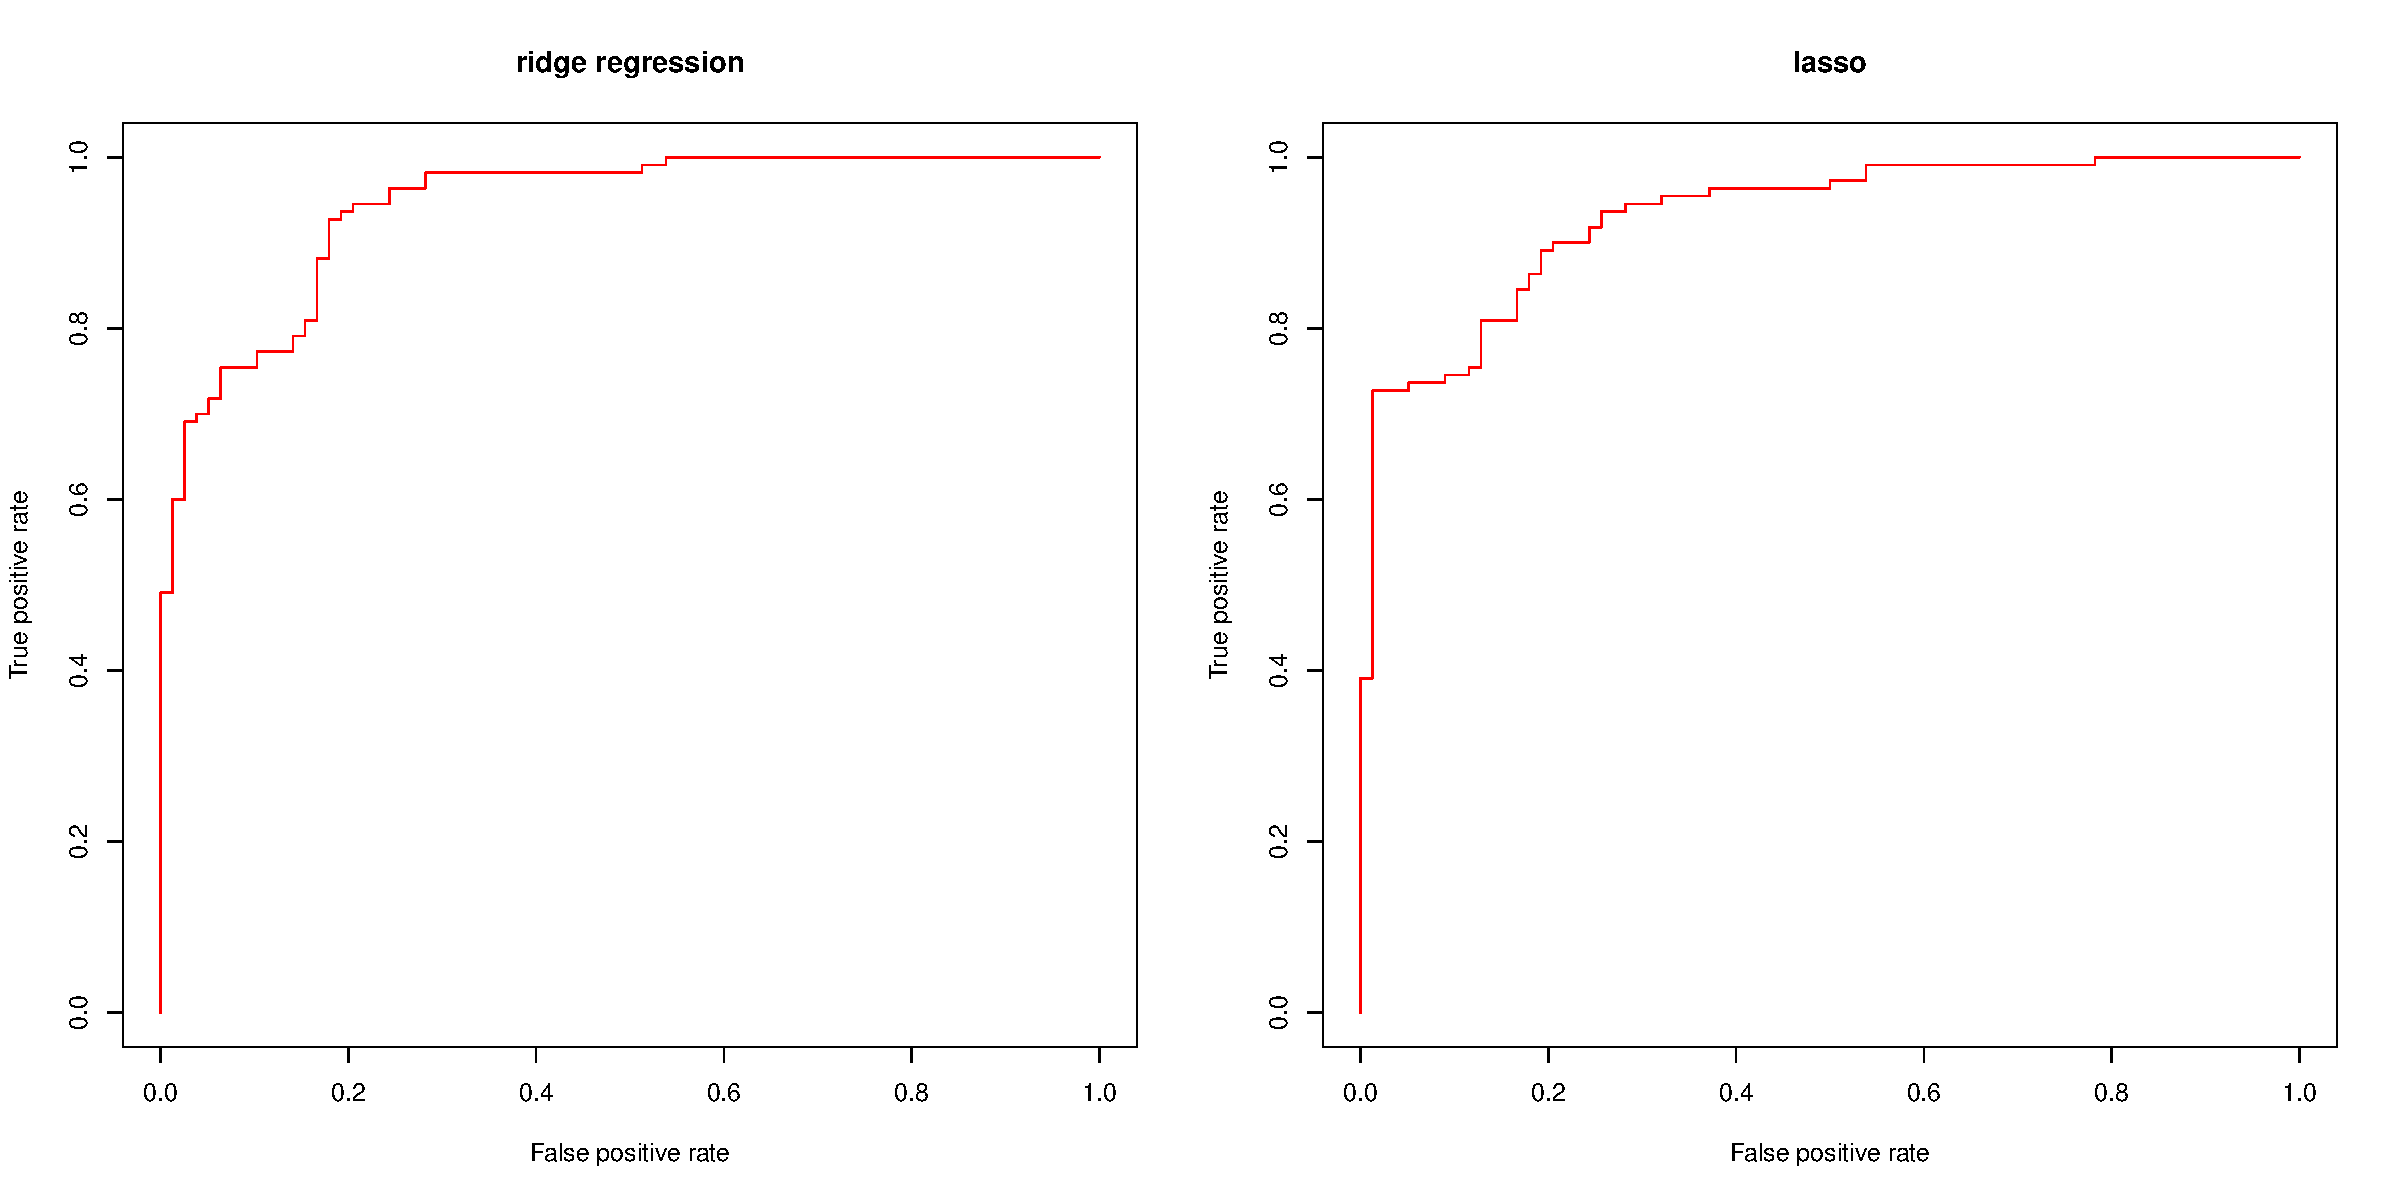
\includegraphics[scale=0.4]{roc-lasso-ridge.pdf}

\end{document}
